\chapter{Implementacja i wyniki}
\thispagestyle{chapterBeginStyle}
\label{chapter5}


Ten rozdział zawiera szczegółowe informacje na temat wykorzystywanych technologii, struktury aplikacji i skryptu, architektury wytrenowanych modeli oraz wyników podsumowujących możliwości wytrenowanych sieci neuronowych.


\section{Opis technologii}
W projekcie wykorzystano język Python 3 \cite{Python}. Python jest interpretowanym, wysokopoziomowym jezykiem  ogólnego zastosowania, o czytelnej, klarownej i zwięzłej składni. Umożliwia programowanie w wielu paradygmatach. Paradygmaty obiektowy i funkcyjny okazały się szczególnie przydatne w trakcie rozwoju projektu. Python jest dynamicznie typowany oraz ma wbudowany garbage collector do zarządzania pamięcią. Często wykorzystywany jest jako język skryptowy. Został wybrany do tego projektu głównie z uwagi na to, że jest on też językiem szeroko wykorzystywanym w kontekście uczenia maszynowego, przez co posiada solidną bazę bibliotek i przydatnych narzędzi.

Jednym z nich jest framework Keras \cite{Keras}, który został wykorzystany do zaimplementowania modelu sieci neuronowej. Zdecydowano się na ten wybór ze względu na prostotę jego nauki i użytkowania, ale też z uwagi na to, że jest to framework powszechnie używany, co ułatwia wyszukiwanie potrzebnych informacji w internecie. Keras sam w sobie zapewnia tylko wysokopoziomowy interfejs służący do tworzenia modeli uczenia głębokiego. Pakiet ten nie implementuje żadnych niskopoziomowych operacji, takich jak przeprowadzanie działań na tensorach czy różniczkowanie. W tych kwestiach polega na wyspecjalizowanych i silnie zoptymalizowanych bibliotekach obsługujących tensory. Autorzy Keras nie wybrali do tego celu jednej konkretnej biblioteki, tym samym wiążąc z nią implementacje pakietu. Zamiast tego, problem ten został rozwiązany modułowo, a więc Keras może użyć jednej z kilku bibliotek jako swojego silnika bazowego. Są to na przykład TensorFlow od Google \cite{TensorFlow}, Theano \cite{Theano} czy Microsoft Cognitive Toolkit (CNTK) \cite{CNTK}. Kod napisany w Keras może być uruchomiony na dowolnej platformie wybranej spośród tych trzech, bez żadnej modyfikacji. Platformę można zmienić w dowolnym momencie pracy, co przydaje się, gdy któraś z nich okazuję się szybsza podczas rozwiązywania problemu.

W projekcie skorzystano z TensorFlow, czyli biblioteki opensource wspierającej trenowanie głębokich sieci neuronowych. TensorFlow pozwala na korzystanie z możliwości nie tylko procesorów CPU, ale też GPU. W tym pierwszym przypadku obudowuje niskopoziomową bibliotekę operacji tensorowych Eigen \cite{Eigen}, natomiast w przypadku procesorów graficznych, TensorFlow stanowi interfejs dla wysoce zoptymalizowanej biblioteki uczenia głębokiego Nvidia CUDA Deep Neural Network (cuDNN) \cite{cuDNN}.

Kod uczenia głębokiego, z uwagi na ogrom operacji przeprowadzanych na tensorach, wykonuje się zdecydowanie szybciej na procesorach graficznych. Jest to szczególnie zauważalne  w przypadku trenowania konwolucyjnych sieci neuronowych. Podczas pracy nad projektem, przejście z CPU Intel Core i5-7300HQ 2.50GHz na procesor graficzny Nvidia GeForce MX150 pozwoliło na skrócenia czasu trenowania modeli od 6 do 10 razy. Z tego powodu instalacja cuDNN jest zdecydowanie zalecana w przypadku dłuższej pracy z aplikacją.


\section{Implementacja}
\subsection{Aplikacja do trenowania sieci}
W celu możliwie jak największego ułatwienia i zautomatyzowania procesu trenowania sieci neuronowych została stworzona aplikacja w języku Python z wykorzystaniem frameworka Keras. Implementacja została oparta w głównej mierze na paradygmacie funkcyjnym, ale wykorzystuje również paradygmat obiektowy. Aplikacja zawiera plik konfiguracyjny \verb|train_config.json| odpowiedzialny za sterowanie nią i procesem trenowania sieci. We wspomnianym pliku należy wyspecyfikować następujące parametry:
\begin{itemize}
    \item \verb|data_directory| - string, ścieżka do bazy danych ze zdjęciami. W katalogu wskazanym przez ten parametr muszą znaleźć się dwa foldery: \verb|train| i \verb|validation|, a każdy z nich musi przechowywać trzy foldery bezpośrednio zawierające zdjęcia w formacie \verb|.jpg|: \verb|positive|, \verb|neutral| i \verb|negative|;
    \item \verb|models_directory| - string, ścieżka do folderu, w którym mają być zapisywane wytrenowane modele;
    \item \verb|results_directory|- string, ścieżka do folderu, w którym mają być zapisywane wyniki trenowania sieci;
    \item \verb|extracted_data_cache_directory| - string, ścieżka do folderu, w którym zapisywany jest cache przyśpieszający trenowania z użyciem transfer learningu;
    \item \verb|use_pretrained_model| - boolean, jeśli true, buduje model z użyciem pretrenowanego modelu wyspecyfikowanego w \verb|pretrained_models|, jeśli false, buduje standardowy model;
    \item \verb|pretrained_model| - string, nazwa uprzednio trenowanego modelu z pakietu Keras, ma zastosowanie tylko, jeśli \verb|use_pretrained_model| jest równe true;
    \item \verb|epochs| - int, liczba iteracji trenowania;
    \item \verb|batch_size| - int, liczba zdjęć na których sieć jest trenowana jednocześnie;
    \item \verb|picture_size| - int, składowa określająca kształt obrazu (rozdzielczość) do jakiego obrazy są sprowadzane w procesie wstępnej obróbki danych, \verb|picture_shape = (picture_size, picture_size)|;
    \item \verb|activation| - string, nazwa funkcji aktywacji wykorzystywanej przez sieć;
    \item \verb|optimizer| - string, nazwa optymalizatora wykorzystywanego przez sieć;
    \item \verb|optimizer_learning_rate| - float, wartość learning\_rate optymalizatora wykorzystywanego przez sieć;
    \item \verb|dropout_rate| - float, współczynnik porzucenia dla warstwy dropout umieszczonej na końcu części konwolucyjnej modelu, określa ułamek wszystkich wartości wejściowych do warstwy, które mają zostać porzucone; 
    \item \verb|kernel_size| - int, składowa określająca kształt jądra konwolucji, \verb|kernel_shape| = (\verb|kernel_size|, \verb|kernel_size|);
    \item \verb|pool_size| - int, składowa określająca wielkość łaty danych wykorzystywanej przez warstwy pooling, \verb|pool_shape = (pool_size, pool_size)|;
    \item \verb|data_augmentation| - boolean, jeśli true, augmentacja danych zostanie wykorzystana, jeśli false, augmentacja danych nie zostanie wykorzystana w trakcie treningu;
    \item \verb|rotation_range| - int, zakres wyrażony w stopniach, o jakie zdjęcie może zostać obrócone podczas augmentacji danych;
    \item \verb|width_shift_range| - float, zakres wyrażony w ułamku całkowitej szerokości, w jakiej zdjęcie może zostać przesunięte w kierunku poziomym podczas augmentacji danych;
    \item \verb|height_shift_range| - float, zakres wyrażony w ułamku całkowitej wysokości, w jakiej zdjęcie może zostać przesunięte w kierunku pionowym podczas augmentacji danych;
    \item \verb|brightness_range| - float, określa stopień, w jakim zdjęcie ma zostać rozjaśnione lub przyciemnione podczas augmentacji danych;
    \item \verb|zoom_range| - float, zakres losowego przybliżenia lub oddalenia obrazu podczas augmentacji danych;
    \item \verb|horizontal_flip| - boolean, jeśli true, zdjęcie może zostać odbite w osi poziomej podczas augmentacji danych, jeśli false, nie może zostać odbite;
    \item \verb|vertical_flip| - boolean, jeśli true, zdjęcie może zostać odbite w osi pionowej podczas augmentacji danych, jeśli false, nie może zostać odbite; 
    \item \verb|fill_mode| - string, definiuje jaki tym wypełnienia ma zostać użyty, gdy podczas augmentacji danym w danym miejscu obrazu nie można wygenerować żadnych pikseli, z uwagi na to, że na obrazie oryginalnym nie istnieje miejsce, które odpowiada temu miejscu. ,,nearest'' oznacza, że w danym miejscu zostanie umieszczony piksel z najbliższej znanej pozycji, która mogła zostać zmapowana. Daje to efekt ,,rozciągnięcia'' obrazu w tym miejscu. ,,reflect'' oznacza lustrzane odbicie obrazu wzdłuż krawędzi ostatnich znanych pikseli. ,,wrap'' oznacza zawijanie obrazu, czyli skopiowanie fragmentu z drugiego końca zdjęcia na to niezajęte pole. Parametr \verb|fill_mode| jest wykorzystywany przy okazji użycia \verb|width_shift|, \verb|height_shift|, ale też \verb|rotation_range|;
    \item \verb|train_line_style| - string, formatuje linię na wykresie dokładności modelu na treningowym zbiorze danych w czasie kolejnych iteracji trenowania;
    \item \verb|validation_line_style| - string, formatuje linię na wykresie dokładności modelu na walidacyjnym zbiorze danych w czasie kolejnych iteracji trenowania;
    \item \verb|info_log| - boolean, jeśli true, wyświetla logi informujące o aktualnych czynnościach podejmowanych przez aplikację;
    \item \verb|model_summary_log| - boolean, jeśli true, przed rozpoczęciem trenowania wyświetla szczegółową architekturę modelu jaki został zbudowany,;
    \item \verb|tensorflow_log| - boolean, jeśli true, wyświetla wszystkie logi standardowo wyświetlane przez TensorFlow.
\end{itemize}
Na podstawie tego pliku tworzony jest obiekt klasy \verb|Config| znajdującej się w pliku \verb|config.py| w pakiecie \verb|config|. Obiekt ten jest dostępny w całej aplikacji, aby za jego pomocą można było wygodnie ją konfigurować i udostępniać dane wprowadzone przez użytkownika poprzez plik \verb|train_config.json|.

Po uruchomieniu pliku \verb|train_main.py|, odwołuje się on do pliku \verb|launch.py| w pakietu \verb|launch|, który jest odpowiedzialny za uruchamianie poszczególnych funkcji z pozostałych pakietów.

Nim aplikacja zbuduje sieć neuronową, przeprowadzana jest wstępna obróbka danych. Odpowiedzialny jest za to pakiet \verb|data|, w którym można znaleźć pliki \verb|preprocessing.py| i \verb|pretrained_preprocessing.py|. Oba są odpowiedzialne za przetwarzanie danych przed wprowadzeniem ich do sieci neuronowej, jednak pierwszy odpowiada za modele zbudowanej w całości przez aplikację, a drugi za te wykorzystujące baze konwolucyjną z uprzednio trenowanego modelu.
W pierwszym przypadku aplikacja wykorzysta dane z odpowiedniej ścieżki, uprzednio te dane augmentując lub nie, w zależności od ustawień obiektu konfiguracyjnego. W drugim przypadku wykorzysta ścieżkę do zcachowanych danych, a jeśli tej ścieżki nie odnajdzie, lub nie odnajdzie cacha zapisanego dla tej konkretnej bazy konwolucyjnej i sposobu preprocessingu danych, skorzysta ze ścieżki do bazy celem stworzenia odpowiedniego cacha.
W pakiecie \verb|data| w pliku \verb|emotion.py| znajduje się klasa \verb|Emotion|, reprezentująca jedną z trzech emocji. W tym samym pakiecie można znaleźć plik \verb|data_set.py|, w którym znajduje się klasa \verb|DataSet|, reprezentująca jeden z trzech zbiorów danych w bazie zdjęć.

W pakiecie \verb|model|, na podstawie architektury wyspecyfikowanej w pliku \verb|preparation.py| oraz przy użyciu obiektu konfiguracyjnego, przygotowywana jest sieć neuronowa. Po stworzeniu i wytrenowaniu tegoż modelu, zostaje on zapisany na dysku w formacie .h5. Oprócz tego, w plikach z rozszerzeniem \verb|.npy| zapisywana jest również historia dokładności osiąganych podczas trenowania. Za obie powyższe funkcjonalności odpowiedzialne są metody znajdujące się w pliku \verb|saving.py| w pakiecie \verb|model|, wykorzystujące obiekt konfiguracyjny (odpowiednio parametry \verb|models_directory| i \verb|results_directory|) w celu zapisywania w żądanej przez użytkownika ścieżce. W tym samym pakiecie znajduje się również plik \verb|visualization.py|, dzięki któremu wyświetlane są wykresy prezentujące dokładność i stratę w kolejnych iteracjach treningu, zarówno dla zbioru walidacyjnego, jak i treningowego.

Ponadto, w pakiecie \verb|utils| znajduje się plik \verb|utils.py|, w którym przechowywane są użyteczne metody wykorzystywane w innych miejscach aplikacji. W tym samym pakiecie tworzony jest też obiekt klasy \verb|Logger|, znajdującej się w pliku \verb|logger.py|. Obiekt ten, podobnie jak obiekt klasy \verb|Config|, jest dostępny w całej aplikacji, ale wykorzystywany jest do informowania użytkownika o aktualnym statusie i akcjach podejmowanych przez aplikacje. Z uwagi na to, że niektóre akcje mogą być czasochłonne, świadomość aktualnego stanu aplikacji pozwoli użytkownikowi uniknąć wrażenia, że aplikacja przestała odpowiadać. Ponadto, w konsoli wypisywana jest też architektura modelu i ostrzeżenia związane z przepełnianiem się pamięci karty graficznej. Wszystkie wyżej wymienione typy logów mogą być wyłączone za pomocą pliku konfiguracyjnego.

\subsection{Skrypt rozpoznający emocje}
W celu wygodnego uruchamiania wytrenowanych sieci dla dowolnych zdjęć i formatowania otrzymanych wyników, został napisany skrypt wykorzystujący plik konfiguracyjny \verb|predict_config.json|.
Użytkownik podczas uruchomienia skryptu może przekazać mu ścieżki do plików lub katalogów zawierających obrazy. Skrypt załaduje wskazany w pliku konfiguracyjnym model, następnie przetworzy te otrzymane pliki, które są w odpowiednim formacie, a ostatecznie zwróci żądane przewidywania w zdefiniowanej przez użytkownika formie. Plik \verb|predict_config.json| pozwala skonfigurować powyższe czynności za pomocą następujących parametrów odpowiedzialnych za sterowanie działaniem skryptu:
\begin{itemize}
    \item \verb|model_path| - string, ścieżka do wytrenowanego modelu zapisanego w formacie \verb|.h5|;
    \item \verb|output_file| - string lub null, jeśli string, wyniki zostaną zapisane do pliku z rozszerzeniem \verb|.json| pod ścieżką zdefiniowaną przez ten parametr. Jeśli parametr nie zostanie podany lub zostanie do niego przypisany null, wyniki zamiast do pliku zostaną wyświetlone w konsoli;
    \item \verb|verbose| - boolean, jeśli false, zostaną wypisane tylko informacje o klasie przewidywanej dla każdego obrazu, jeśli true, oprócz tego zostaną też wypisane informacje o prawdopodobieństwie przynależności obrazu do każdej z klas. Ma zastosowanie zarówno podczas wypisywania wyników w konsoli, jak i podczas zapisu do pliku; 
    \item \verb|info_log| - boolean, jeśli true, wyświetla logi informujące o aktualnych czynnościach podejmowanych przez skrypt;
    \item \verb|tensorflow_log| - boolean, jeśli true, wyświetla wszystkie logi normalnie wyświetlane przez TensorFlow.
\end{itemize}


\section{Model konwolucyjnej sieci neuronowej}
Pierwszym zastosowanym podejściem jest zaimplementowanie od podstaw własnej konwolucyjnej sieci neuronowej i sprawdzenie, jakie wyniki jest ona w stanie osiągnąć. Przygotowywanie danych do pierwszych testów rozpoczęto od modyfikowania rozdzielczości zdjęć w taki sposób, żeby wszystkie były rozmiaru 150x150 pikseli. Obrazy podczas preprocessingu często sprowadza się do tej rozdzielczości z racji tego, że często okazuje się ona być złotym środkiem pomiędzy jakością obrazu, a jego wielkością (czyli jednocześnie ilością danych jakie model musi przetworzyć). Taka rozdzielczość pozwala dość dokładnie określić co dzieje się na zdjęciu, np. człowiek nie ma żadnych problemów z rozpoznawaniem szczegółów na obrazie w takiej rozdzielczości. Jednocześnie zdjęcie składające się z większej liczny pikseli przekłada się na większy tensor, jaki musi być przetworzony przez pierwszą warstwę. Z kolei większy tensor wchodzący do pierwszej warstwy oznacza z reguły (jest to też zależne od architektury sieci), że kolejne tensory również będą większe.
%JL, co w konsekwencji ogólnie przełoży się na większą liczba parametrów do dostrojenia dla danej sieci. 
Wydłuża to czas treningu, a także czas działania modelu. Jest to zdecydowanie niepożądane w przypadku modeli wykorzystywanych na urządzeniach 
o ograniczonych zasobach,  jak np. urządzenia mobilne.
%JL, lecz co gorsza sprawia, że model waży zdecydowanie więcej. Jest to niepożądane w przypadku modeli wykorzystywanych na urządzeniach nie dysponujących dużą ilością miejsca na dysku, jak np. urządzenia mobilne. Z perspektywy użytkownika końcowego taka sieć nie dość, że zajmuje więcej miejsca na dysku, to również dłużej się wczytuje i potrzebuje więcej czasu na przetwarzanie zdjęć. Ponadto, w zbyt dużych sieciach często dochodzi do zjawiska nadmiernego dopasowywania się modelu do danych wejściowych.

Do pierwszego testu wykorzystano architekturę sieci składającą się z czterech bloków, w której każdy blok stanowi parę złożoną z dwóch warstw - warstwy konwolucyjnej o pewnej liczbie filtrów i pewnej funkcji aktywacji oraz warstwy max pooling. Liczby filtrów w każdej następnej warstwie konwolucyjnej wynoszą odpowiednio 32, 64, 128 i 128. Celem takiej zwężającej się, ale coraz głębszej architektury jest ułatwienie sieci tworzenia hierarchii wzorców przestrzennych (patrz rozdział (\ref{chapter4}). Każda z warstw konwolucyjnych wykorzystuje jądra o standardowym rozmiarze równym 3x3. Każda z warstw max pooling również jest sparametryzowana w standardowy sposób, to znaczy używa okien konwolucyjnych o rozmiarze 2x2 i przesuwa je z krokiem równym 2. Można łatwo obliczyć, że ostatnia warstwa w tak zbudowanej bazie konwolucyjnej ma rozmiar (7, 7, 128). Do niej zostały dopięte jeszcze dwie warstwy gęste, wewnętrzna o 512 neuronach i wyjściowa o 3 neuronach reprezentujących 3 klasy wyjściowe. Z uwagi na to, że rozwiązywany jest problem klasyfikacji wieloklasowej, gdzie każdy obraz przypisywany jest do dokładnie jednej klasy, ostatnia warstwa korzysta z funkcji softmax, dzięki czemu suma wartości wyjściowych na tych trzech neuronach wynosi 1, co może być interpretowane jako prawdopodobieństwo, stopień pewności sieci o przynależności rozpatrywanego zdjęcia do danej klasy. Jako funkcja straty została wykorzystana kategorialna entropia krzyżowa.

Przeprowadzono 8 testów, z wykorzystaniem 4 różnych funkcji aktywacji: ReLU, tangensa hiperbolicznego (tanh), sigmoid i softmax. Dla każdej z tych funkcji model został skompilowany dwa razy za pomocą dwóch różnych optymalizatorów: RMSProp i Adam, oba parametryzowane learning rate równym $10^{-4}$. RMSProp (Root Mean Square Propagation) został wybrany z uwagi na to, że jest to optymalizator często wykorzystywany w problemach klasyfikacji obrazów. Przewagą Adam (Adaptive Moment Estimation) z kolei jest to, że charakteryzuje się on krótszym czasem osiągania dobrych wyników, jednakże w niektórych problemach klasyfikacji obrazów może nie być w stanie osiągnąć rozwiązania optymalnego.

Dokładności osiągnięte przez sieci na walidacyjnym zbiorze danych po 15 iteracjach trenowania zostały przedstawione w tabeli \ref{tab:5.1}.

\begin{table}[H]
  \caption{Dokładności osiągnięte po 15 iteracjach trenowania dla opisywanego modelu przetwarzającego zdjęcia w rozmiarze 150x150.}
    \centering
    \begin{tabular}{ |c|c|c| }
    \hline
    Sieć & RMSProp($10^{-4}$) & Adam($10^{-4}$) \\
    \hline
    ReLU & 40.2\% & \textbf{45.2\%} \\
    Tanh & 40.2\% & \textbf{47.7\%} \\
    Sigmoid & 40.4\% & 40.2\% \\
    Softmax & 40.2\% & 40.2\% \\
    \hline
    \end{tabular}
  \label{tab:5.1}
\end{table}

W tabeli \ref{tab:5.1} pogrubioną czcionką zaznaczono wyniki wyraźnie lepsze od reszty. Już po pierwszym rzucie oka nasuwa się pytanie - dlaczego zdecydowana większość sieci osiągnęła identyczne lub niemal identyczne wyniki, w okolicach 40.2\%? Wykresy przedstawiające historie dokładności osiąganej na walidacyjnym zbiorze danych (przykład dla funkcji sigmoid i optymalizatora ADAM przedstawiono na wykresie \ref{pic:5.1}) wskazują na to, że większość z tych sieci osiągnęła tę wydajność już po pierwszej lub drugiej iteracji. Natomiast w przypadku zbioru testowego sieci z reguły bardzo szybko osiągały wyniki na poziomie 40.5\%. Przyjrzenie się bazie danych pokazuje, że liczba zdjęć przedstawiających emocje pozytywne w zbiorze walidacyjnym wynosi 40.2\% wszystkich zdjęć w tym zbiorze, natomiast w przypadku zbioru treningowego analogiczna wartość wynosi 40.5\% (zobacz rozdział \ref{chapter4}). W obu przypadkach jest to podzbiór większy od podzbiorów zdjęć emocji neutralnych czy negatywnych. Sugeruje to więc, że sieci wpadały w swego rodzaju lokalne maksima, zawsze zakładając, że na zdjęciu wyrażone są emocje pozytywne, ponieważ podczas treningu właśnie taka odpowiedź miała największe szanse na bycie odpowiedzią poprawną.

\begin{figure}[H]
    \caption{Historia wydajności przy zastosowaniu funkcji aktywacji sigmoid i optymalizatora Adam.}
    \centering
    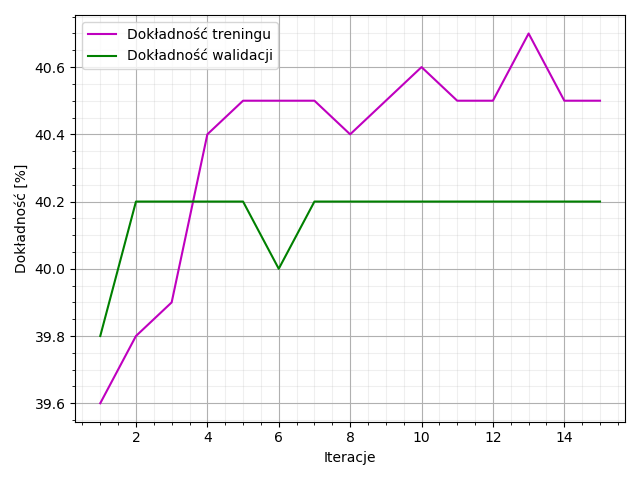
\includegraphics[width=0.7\textwidth]{wykres1.png}
    \label{pic:5.1}
\end{figure}

Po uruchomieniu tych sieci i przekazaniu do klasyfikacji całego zbioru testowego oraz walidacyjnego okazało się to prawdą - sieci niemal w każdym przypadku rozpoznawały emocje pozytywną. Co więcej, nierzadko robiły to z niemal stuprocentową pewnością. Sieci utykały więc w lokalnym maksimum.

Dalsze testy z wykorzystaniem optymalizatora RMSProp nie dały lepszych wyników- niezależnie od wybranej funkcji aktywacji i niezależnie od wykorzystanego learning rate (który przyjmował wartości od $10^{-1}$ do $10^{-7}$), wszystkie sieci z użyciem tego optymalizatora uzyskały wyniki równe 40.2\% lub nawet gorsze (w przypadku najniższych learning rate). Podobnie rzecz miała się w przypadku optymalizatora Adam w połączeniu z funkcjami aktywacji sigmoid lub softmax, żaden test nie wykazał przekroczenia ,,granicy'' 40.2\%.

Jednak połączenie optymalizatora Adam z funkcjami aktywacji ReLu i tanh zasługuje na szczególną uwagę. Obie te architektury również zostały przetestowano dla różnych learning rate. Każdy test przeprowadzono dla 15 cykli trenowania. Wyniki tych testów zostały przedstawione w tabeli \ref{tab:5.2}.

\begin{table}[H]
  \centering
  \caption{Dokładności osiągnięte po 15 iteracjach trenowania dla modelu kompilowanego z użyciem optymalizatora Adam.}
    \begin{tabular}{ |c|c|c| }
    \hline
    Learning rate & ReLU & Tanh \\
    \hline
    $10^{-3}$ & 40.2\% & 40.2\% \\
    $10^{-4}$ & \textbf{45.2\%} & \textbf{47.4\%} \\
    $10^{-5}$ & \textbf{44.1\%} & \textbf{50.9\%} \\
    $10^{-6}$ & 40.2\% & \textbf{47.7\%} \\
    $10^{-7}$ & 40.2\% & 40.2\% \\
    \hline
    \end{tabular}
  \label{tab:5.2}
\end{table}

We wszystkich przypadkach 15 epok trenowania wystarczyło, by sieci osiągnęły maksimum swojej dokładności na zbiorze walidacyjnym- z reguły osiągały ją już w okolicach od 5. do 8. iteracji. Na wykresie \ref{pic:5.2} przedstawiono przykładową historie treningu dla funkcji aktywacji tanh i optymalizatora Adam z learning rate wynoszącym $10^{-5}$. Dalej można zaobserwować poprawę dokładności tylko dla zbioru treningowego- klasyczne nadmierne dopasowanie. By rozwiązać ten problem, w następnym podrozdziale zostanie wykorzystana augmentacja danych, by spróbować jeszcze ulepszyć te modele, które już do tej pory wypadły najlepiej, tj. np. model z funkcją aktywacji tanh dla learning rate równego $10^{-5}$ czy model wykorzystujący ReLU z learning rate równym $10^{-4}$.

\begin{figure}[H]
    \caption{Historia wydajności przy zastosowaniu funkcji aktywacji tanh i optymalizatora Adam z learning rate wynoszącym $10^{-5}$}
    \centering
    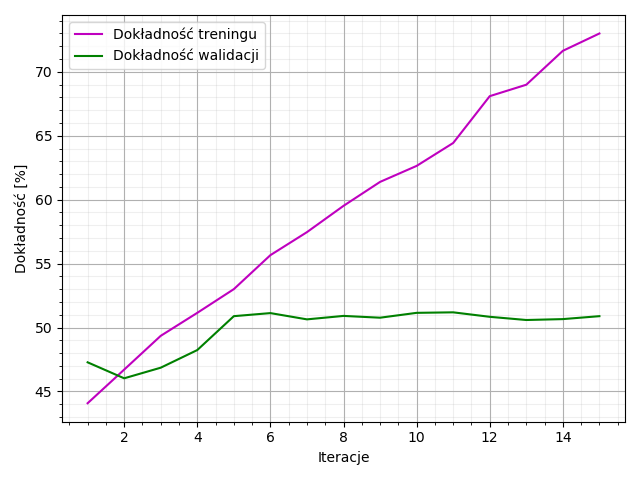
\includegraphics[width=0.7\textwidth]{wykres2.png}
    \label{pic:5.2}
\end{figure}

Każdy z dotychczas wytrenowanych modeli (z uwagi na podobną architekturę) waży tyle samo, tj. 39.5 MB, dzięki czemu nie powinno być większych problemów z wykorzystywaniem takich sieci w aplikacjach przeznaczonych na różne rodzaje sprzętu, w tym urządzenia mobilne. W celu sprawdzenia, czy inna głębokość warstw poprawi wydajność modelu, kolejnym krokiem jest przeprowadzenie testów dla sieci składających się z innych liczb filtrów wykorzystywanych przez te warstwy. Przypomnijmy, że wyjściowa architektura składała się z czterech par warstw, z których każda złożona była z warstwy konwolucyjnej i max pooling. Liczba filtrów w warstwach konwolucyjnych wynosiła odpowiednio: 32, 64, 128, 128. Do kolejnych testów zbudowano 3 nowe sieci o następujących liczbach filtrów, sieć A: 16, 32, 64, 64; sieć B: 16, 32, 64, 128; oraz sieć C: 32, 64, 128, 256. Każdy model skompilowano kilka razy za pomocą optymalizatora Adam z learning rate na takim poziomie, które w poprzednich testach zapewniało najlepszą wydajność. Wykorzystano również funkcje aktywacji z najlepszymi do tej pory wynikami, tj. ReLu i tanh. Każdy model był trenowany przez 15 epok. Wyniki tych testów zamieszczono w tabeli \ref{tab:5.3}.

\begin{table}[H]
  \centering
  \caption{Dokładności osiągnięte po 15 iteracjach trenowania dla modeli o różnych liczb filtrów}
    \begin{tabular}{ |c|c|c|c|c|c| }
    \hline
    F. aktywacji & L. rate & Model wyjściowy & Model A & Model B & Model C \\
    \hline
    ReLU & $10^{-4}$ & 45.2\% & 44.5\% & 45.0\% & 45.0\% \\
    ReLU & $10^{-5}$ & 44.1\% & 43.6\% & 43.6\% & 44.3\% \\
    ReLU & $10^{-6}$ & 40.2\% & 40.2\% & 40.2\% & 40.2\% \\
    Tanh & $10^{-4}$ & 47.4\% & 47.0\% & 47.2\% & 47.5\% \\
    Tanh & $10^{-5}$ & \textbf{50.9\%} & \textbf{50.4\%} & \textbf{50.4\%} & \textbf{50.7\%} \\
    Tanh & $10^{-6}$ & 47.7\% & 47.4\% & 47.3\% & 47.8\% \\
    \hline
    \end{tabular}
  \label{tab:5.3}
\end{table}

Testy wykazują, że zwiększanie liczby filtrów nie zdaje egzaminu- model C osiągnął wyniki niemal identyczne z modelem wyjściowym, co czyni go gorszym rozwiązaniem- ten model, z uwagi na większą liczbę parametrów do wytrenowania, potrzebował więcej czasu na osiągnięcie pełnej wydajności, a jednocześnie zajmuje niemal dwukrotnie więcej miejsca na dysku (78 MB). Lżejsze modele o mniejszej liczbie filtrów, tj. A (19.1 MB) i B (37.9 MB) uzyskały wyniki podobne do siebie, a jednocześnie niewiele gorsze od wyników uzyskanych przez model wyjściowy. Jednak z uwagi na to, że są lżejsze, zdają się być warte dalszej analizy z uwzględnieniem augmentacji danych (szczególnie ponad dwukrotnie mniejszy model A).

Kolejne testy zostały przeprowadzone z wykorzystaniem jąder konwolucji o większym rozmiarze- 5x5. Wykonano je dla kilku modeli wybranych z poprzednich rozważań. W tabeli \ref{tab:5.4} zamieszczono porównanie wyników w przypadku użycia jąder konwolucji o rozmiarze 3x3 i 5x5.

\begin{table}[H]
  \centering
  \caption{Dokładności osiągnięte po 15 iteracjach trenowania dla modeli o różnych wielkościach jąder konwolucji}
    \begin{tabular}{ |c|c|c|c|c| }
    \hline
    F. aktywacji & L. rate & Model & Kernel 3x3 & Kernel 5x5 \\
    \hline
    Tanh & $10^{-5}$ & Model wyjściowy & \textbf{50.9\%} & 49\% \\
    Tanh & $10^{-5}$ & Model C & \textbf{50.7\%} & 48.4\% \\
    Tanh & $10^{-6}$ & Model C & 47.8\% & 46.1\% \\
    ReLU & $10^{-4}$ & Model wyjściowy & 45.2\% & 44.6\% \\
    \hline
    \end{tabular}
  \label{tab:5.4}
\end{table}

W każdym z przetestowanych przypadków wykorzystanie mniejszego jądra konwolucji zapewnia nieznacznie lepsze wyniki. Z drugiej strony, większe jądro konwolucji sprawia, że wysokość i szerokość analizowanego tensora spada szybciej z warstwy na warstwę, przez co modele z jego wykorzystaniem są lżejsze. Dla przykładu, model wyjściowy o jądrze konwolucji rozmiaru 3x3 waży 39.5 MB, podczas gdy model o tej samej architekturze, ale z jądrem konwolucji rozmiaru 5x5 waży 26.4 MB.

Następnym krokiem jest przeprowadzenie testów z wykorzystaniem modeli zaprojektowanych do analizy zdjęć o rozdzielczości 224x224 pikseli. Większa rozdzielczość zdjęć wejściowych wydłuży proces trenowania i zwiększy wagę modelu, jednakże może również zwiększyć dokładność przewidywań, jeśli okaże się, że sieć jest w stanie dostrzec szczegóły obrazu, których nie dostrzegła na mniejszych zdjęciach.

Pierwszy zaprojektowany model złożony jest z czterech bloków warstw. W skład pierwszych dwóch bloków wchodzą po dwie warstwy konwolucyjne i jedna warstwa max pooling. Na ostatnie dwa bloki składają się 3 warstwy konwolucyjne i jedna warstwa max pooling. Liczby filtrów w każdej warstwie konwolucyjnej w danym bloku jest taka sama i wynosi odpowiednio 32, 64, 128 i 128 w kolejnych blokach. Tak samo jak w przypadku poprzednich modeli przetwarzających mniejsze zdjęcia, tak i teraz, każda z warstw max pooling jest sparametryzowana w standardowy sposób, to znaczy używa okien konwolucyjnych o rozmiarze 2x2 i przesuwa je z krokiem równym 2. Warstwy konwolucyjne również wykorzystują jądra o standardowym rozmiarze równym 3x3. Można obliczyć, że ostatnia warstwa w tak zbudowanej bazie konwolucyjnej ma rozmiar (8, 8, 128). Z uwagi na to, że jest to rozmiar podobny do tego z modelu dla mniejszych zdjęć, zostanie dopięty podobny klasyfikator, o dwóch warstwach gęstych, wewnętrznej o 512 neuronach i wyjściowej o trzech neuronach reprezentujących 3 klasy wyjściowe. Ostatnia warstwa będzie używać funkcji aktywacji softmax. Jako funkcja straty została wykorzystana kategorialna entropia krzyżowa.

Wykonano 8 testów, z wykorzystaniem 4 różnych funkcji aktywacji: ReLU, tanh, sigmoid i softmax. Dla każdej z tych funkcji model był kompilowany wielokrotnie za pomocą dwóch różnych optymalizatorów: RMSProp i Adam, oba z learning rate z przedziału od $10^{-7}$ do $10^{-3}$. Testy przeprowadzone na tym modelu dały rezultaty bardzo podobne do tych przeprowadzonych na sieci dostosowanej do analizy zdjęć w rozdzielczości 150x150. Zarówno optymalizator RMSProp i funkcje sigmoid i softmax są nieodpowiednie do tego zadania, po raz kolejny modelom je wykorzystującym nie udało im się wyjść z lokalnego maksimum. Funkcje tanh i ReLU poradziły sobie lepiej, ale wciąż nie tak dobrze, jak w przypadku modelu wykorzystywanego do analizy zdjęć w rozdzielczości 150x150 pikseli. Najlepsze wyniki przedstawiono w tabeli \ref{tab:5.5}. Nie uwzględniono tam sieci osiągających najsłabsze rezultaty.

\begin{table}[H]
  \centering
  \caption{Dokładności osiągnięte po 20 iteracjach trenowania dla modelu kompilowanego z użyciem optymalizatora Adam i analizującego zdjęcia w rozmiarze 224x224 pikseli}
    \begin{tabular}{ |c|c|c| }
    \hline
    Learning rate & ReLU & Tanh \\
    \hline
    $10^{-4}$ & 44.7\% & 43.4\% \\
    $10^{-5}$ & \textbf{47.7\%} & \textbf{47.7\%} \\
    $10^{-6}$ & 40.2\% & \textbf{49.1\%} \\
    \hline
    \end{tabular}
  \label{tab:5.5}
\end{table}

Można zauważyć, że rozkład wyników jest bardzo podobny do przypadku, w którym analizowane były sieci dla zdjęć rozdzielczości 150x150. Trening sieci tym razem wymaga jednak większej liczby cykli, jednakże w każdym przypadku 20 iteracji wystarczyło, by modele osiągnęły pełnie swoich możliwości. Na wykresie \ref{pic:5.3} przedstawiono historie treningu modelu, który osiągnął najlepsze rezultaty, tj. wykorzystującego funkcję aktywacji tanh i optymalizator Adam z learning rate wynoszącym $10^{-6}$. Można zaobserwować, że od pewnego momentu wydajność wzrasta już tylko dla zbioru treningowego. Ten problem można częściowo rozwiązać za pomocą augmentacji danych, jednakże zdaje się, że wcześniej rozpatrywane modele były bardziej warte uwagi w tej kwestii, szczególnie biorąc pod uwagę, że nowe modele zajmują zdecydowanie więcej miejsca na dysku, ponieważ każdy z nich waży 58.1 MB.

\begin{figure}[H]
    \caption{Historia wydajności przy zastosowaniu funkcji aktywacji tanh i optymalizatora Adam z learning rate wynoszącym $10^{-6}$}
    \centering
    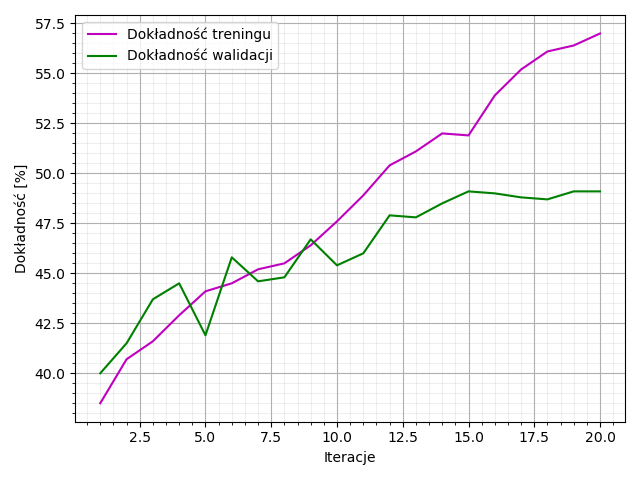
\includegraphics[width=0.7\textwidth]{wykres3.png}
    \label{pic:5.3}
\end{figure}

Przed wykonaniem testów z wykorzystaniem augmentacji danych, zostaną jeszcze przeprowadzone modyfikacje liczby filtrów wykorzystywanych przez warstwy w celu sprawdzenia, czy inna głębokość warstw poprawi wydajność modelu. Przypomnijmy, że wyjściowa architektura składała się z czterech bloków warstw, z których każdy złożony był z dwóch albo trzech warstw konwolucyjnych i jednej warstwy max pooling. Liczba filtrów w warstwach konwolucyjnych tego samego bloku była taka sama i wynosiła odpowiednio: 32, 64, 128, 128 dla kolejnych bloków. Do kolejnych testów zbudowano 3 nowe sieci o następujących liczbach filtrów, sieć A: 16, 32, 64, 128; sieć B: 32, 64, 128, 256; sieć C: 64, 128, 256, 256. Wyniki wydajności osiągniętych przez nowe modele kompilowane za pomocą optymalizatora Adam zostały przedstawione w tabeli \ref{tab:5.6}.

\begin{table}[H]
  \centering
  \caption{Dokładności osiągnięte po 20 iteracjach trenowania dla modeli kompilowanych z użyciem optymalizatora Adam}
    \begin{tabular}{ |c|c|c|c|c|c| }
    \hline
    F. aktywacji & L. rate & Model wyjściowy & Model A & Model B & Model C \\
    \hline
    ReLU & $10^{-4}$ & 44.7\% & 42.4\% & 41.5\% & 41.7\% \\
    ReLU & $10^{-5}$ & 47.7\% & 45.0\% & \textbf{49.3}\% & \textbf{48.2}\% \\
    ReLU & $10^{-6}$ & 40.2\% & 40.2\% & 40.2\% & 40.2\% \\
    Tanh & $10^{-4}$ & 43.4\% & 42.1\% & 43.2\% & 43.4\% \\
    Tanh & $10^{-5}$ & 47.7\% & 45.8\% & 44.7\% & 47.8\% \\
    Tanh & $10^{-6}$ & \textbf{49.1}\% & 47.5\% & \textbf{48.2}\% & \textbf{49.2}\% \\
    \hline
    \end{tabular}
  \label{tab:5.6}
\end{table}

W tym przypadku zwiększenie liczby filtrów pomogło w niektórych konfiguracjach- widać to wyraźnie dla funkcji aktywacji ReLU i learning rate o wartości $10^{-5}$. Wydajność w tym przypadku dla modelu B wzrosła o 1.6 p.p., jednakże jest on cięższy, bo waży aż 117 MB, co w zasadzie wyklucza go z dalszych rozważań. W pozostałych przypadkach modele B i C w większości osiągnęły wyniki porównywalne do tych osiągniętych przez model wyjściowy, ale z uwagi na, że są zdecydowanie cięższe (model C waży aż 136 MB) nie będą dalej rozważane. Z kolei modele o mniejszej głębokości warstw radziły sobie widocznie słabiej, najwidoczniej mała liczba filtrów nie pozwoliła wykształcić tak dobrej hierarchii cech.


\section{Augmentacja danych}
Kolejny etap ulepszania modeli opiera się na wykorzystaniu augmentacji danych. W rozdziale \ref{chapter4}. zostały opisane modyfikacje obrazów, które zostaną zastosowane w celu wzbogacania zbioru zdjęć. Z uwagi na zdecydowanie większą ilość czasu potrzebną do trenowania sieci z wykorzystaniem tej techniki, testy zostaną przeprowadzone na tych modelach, które w poprzednim podrozdziale uzyskały najlepszą dokładność na walidacyjnym zbiorze danych.

W pierwszym teście augmentacja zostanie przeprowadzona z następującymi argumentami opisanymi na początku tego rozdziału: rotation\_range = 40, width\_shift = 0.2, height\_shift = 0.2, brightness\_range = 0.2, zoom\_range = 0.2, horizontal\_flip = true, vertical\_flip = false, fill\_mode =,,nearest'' i dropout\_rate = 0.5. Jest to często wykorzystywana konfiguracja. Tabela \ref{tab:5.7} przestawia porównanie wydajności sieci, które w poprzednim podrozdziale dawały najlepsze wyniki, tym razem trenowane w 80 iteracjach z wykorzystaniem augmentacji i bez niej. Wszystkie z testowanych modeli przetwarzały zdjęcia w rozmiarze 150x150 i używały optymalizatora Adam.
\begin{table}[H]
  \centering
  \caption{Dokładności osiągnięte po 80 iteracjach trenowania dla modeli, które osiągnęły najlepsze rezultaty bez augmentacji danych}
    \begin{tabular}{ |c|c|c|c|c| }
    \hline
    F. aktywacji & L. rate & Model & Bez augmentacji & Z augmentacją \\
    \hline
    Tanh & $10^{-5}$ & Model wyjściowy & 50.9\% & 52.4\% \\
    Tanh & $10^{-5}$ & Model C & 50.7\% & 52.7\% \\
    Tanh & $10^{-6}$ & Model C & 47.8\% & 50.1\% \\
    ReLU & $10^{-4}$ & Model wyjściowy & 45.2\% & \textbf{54.8}\% \\
    \hline
    \end{tabular}
  \label{tab:5.7}
\end{table}

Zgodnie z oczekiwaniami, augmentacja danych poprawiła wydajność w przypadku każdej sieci, jednak na szczególną uwagę zasługuje tutaj sieć wykorzystująca funkcję ReLU w charakterze funkcji aktywacji. W tym przypadku wydajność osiągnęła 54.8\% na walidacyjnym zbiorze danych, co jest najlepszym wynikiem do tej pory. W stosunku do tego samego modelu nie wykorzystującego augmentacji danych, wydajność poprawiła się o 9.6 p.p, czyli aż o 21\% w skali względnej. Historię trenowania tej sieci przedstawiono na wykresie \ref{pic:5.4}. 
\begin{figure}[H]
    \caption{Historia wydajności przy zastosowaniu funkcji aktywacji ReLU i augmentacji danych.}
    \centering
    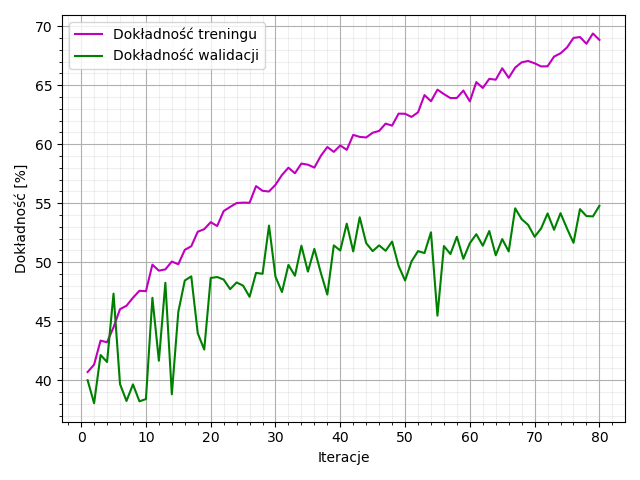
\includegraphics[width=0.7\textwidth]{wykres4.png}
    \label{pic:5.4}
\end{figure}
Można zauważyć, że wykresy wykorzystujące augmentacje danych zachowują się inaczej niż te, które tego nie robią. Te ostatnie zdecydowanie szybciej osiągają pełną wydajność dla zbioru treningowego (przetrenowanie), a jeszcze szybciej dla zbioru walidacyjnego (brak rzeczywistego treningu z uwagi na zbytnie dostosowanie do zbioru treningowego). W przypadku modelu wykorzystującego augmentacje danych, linie zdają się być bardziej skorelowane ze sobą. Mimo tego, że wartości nie są podobne do siebie, to dokładność dla zbioru walidacyjnego rośnie stale wraz z dokładnością dla zbioru treningowego. Na wykresie można zobaczyć, że mimo wykonania 80 cyklu trenowania, dokładność treningu nawet nie zbliżyła się do 100\%, chociaż widać pewne oznaki przetrenowania (wartości coraz bardziej odbiegają od tych dla zbioru walidacyjnego). Jednakże, dokładność walidacji stale rośnie i wydaję się prawdopodobne, że np. kolejne kilkadziesiąt iteracji pozwoliło by zwiększyć wydajność jeszcze o kilka punktów procentowych. Wykorzystanie augmentacji danych nie ma wpływu na ilość miejsca, jaką sieć zajmuje na dysku, ponieważ augmentacja danych modyfikuje tylko dane treningowe, w żaden sposób nie wpływając na kształt architektury sieci. Z tego powodu model, którego historia trenowania została przedstawiona, waży 39.5 MB, czyli dokładnie tyle samo, co odpowiadający mu model opisywany w poprzednim rozdziale.

W przypadku modeli wykorzystujących funkcję tanh w charakterze funkcji aktywacji, ostateczna dokładność walidacji z użyciem augmentacji danych wzrosła w najlepszym przypadku tylko o około 2 p.p. Może to częściowo wynikać z faktu, że funkcja tanh już wcześniej osiągała lepszą wydajność, więc niewątpliwie ciężej było jeszcze bardziej ją zwiększyć. Jednakże trzeba też zauważyć, że funkcja ReLU, mimo tego, że w analizowanym zestawieniu bez augmentacji danych osiągała najgorsze wyniki, po użyciu augmentacji stała się najbardziej wydajna.

Z tego powodu, w kolejnych testach zostaną wzięte pod uwagę inne modele wykorzystujące funkcję ReLU. Testy zostaną przeprowadzone dla różnych wartości parametru \verb|dropout_rate|. Ma to na celu wyrównanie dokładności dla zbioru treningowego i walidacyjnego, ponieważ w poprzednim teście wartości te coraz bardziej różniły się od siebie w kolejnych iteracjach. Wyniki zostały przedstawione w tabeli \ref{tab:5.8}.

\begin{table}[H]
  \centering
  \caption{Dokładności osiągnięte po 80 iteracjach trenowania z wykorzystaniem różnych wartości współczynnika porzucenia.}
    \begin{tabular}{ |c|c|c|c|c|c|c|c| }
    \hline
    \multirow{2}{*}{F. akt.} & \multirow{2}{*}{L. rate} & \multirow{2}{*}{Model} & \multirow{2}{*}{Rozmiar} & \multirow{2}{*}{Bez aug.} & \multicolumn{3}{c|}{Z augmentacją} \\
    \cline{6-8}
    &&&&& Dropout 0.5 & Dropout 0.35 & Dropout 0.6 \\
    \hline
    ReLU & $10^{-4}$ & M. wyjściowy & 150x150 & 45.2\% & \textbf{54.8\%} & 51.9\% & 40.2\% \\
    ReLU & $10^{-5}$ & M. wyjściowy & 150x150 & 44.1\% & \textbf{51.5\%} & 50.6\% & 40.2\% \\
    
    ReLU & $10^{-4}$ & M. wyjściowy & 224x224 & 44.7\% & \textbf{50.2\%} & 46.9\% & 40.2\% \\
    ReLU & $10^{-5}$ & Model B & 224x224 & 49.3\% & \textbf{54.6\%} & 49.6\% & 40.2\% \\
    \hline
    \end{tabular}
  \label{tab:5.8}
\end{table}

Okazuje się, że podniesienie współczynnika porzucenia do 0.6 całkowicie uniemożliwia sieci wykształcenie przestrzennej hierarchii wzorów. Lepiej sprawdza się obniżenie \verb|dropout_rate|, ale tutaj z kolei ponownie pojawia się problem nadmiernego dopasowania- dokładność treningowa rośnie szybciej, niż w przypadku \verb|dropout_rate| = 0.5, osiągając ostatecznie wartości bliskie 100\%, jednocześnie uniemożliwiając tym samym wykształcenie cech, które przydałyby się podczas analizy zdjęć nie wchodzących w skład zbioru treningowego. Obniżenie wartości \verb|dropout_rate| wypada szczególnie słabo w przypadku sieci analizujących zdjęcia w rozmiarze 224x224.

W ostatnim teście została użyta sieć, która do tej pory osiągała najlepsze wyniki, tj. model wyjściowy analizujący zdjęcia w rozdzielczości 150x150 z wykorzystaniem ReLU w charakterze funkcji aktywacji oraz optymalizatora Adam o wartości learning rate wynoszącej $10^{-4}$. Test zakłada modyfikowanie parametrów augmentacji. Wyniki zostały przedstawione w tabeli \ref{tab:5.9}.

\begin{table}[H]
  \centering
  \caption{Dokładności osiągnięte po 80 iteracjach trenowania z wykorzystaniem różnych współczynników augmentacji.}
    \begin{tabular}{ |c|c|c|c|c|c|c|c| }
    \hline
    rotation\_r. & width\_s. & height\_s. & brightness\_r. & zoom\_r. & horizontal\_f. & fill\_m. & Dokładność \\
    \hline
    40 & 0.2 & 0.2 & 0.2 & 0.2 & true & ,,nearest'' & \textbf{54.8}\% \\
    30 & 0.15 & 0.15 & 0.15 & 0.15 & false & ,,nearest'' & 54.4\% \\
    50 & 0.25 & 0.25 & 0.25 & 0.25 & true & ,,nearest'' & 46.9\% \\
    0 & 0.25 & 0.25 & 0.25 & 0.25 & true & ,,nearest'' & 48.1\% \\
    40 & 0.2 & 0.2 & 0.2 & 0.2 & true & ,,reflect'' & \textbf{55.1}\% \\
    40 & 0.2 & 0.2 & 0.2 & 0.2 & true & ,,wrap'' & \textbf{54.9}\% \\
    \hline
    \end{tabular}
  \label{tab:5.9}
\end{table}

Testy wykazały, że w przypadku obniżenia wartości argumentów, sytuacja ma się bardzo podobnie, jak w przypadku zastosowania argumentów wyjściowych- wyniki są tylko nieznacznie słabsze. Z kolei zwiększenie ,,siły'' augmentacji wpływa negatywnie na zdolność uczenia się modelu- co prawda nie występuje problem przetrenowania, ale mimo 80 iteracji nauki, sieci nie udało się wykształcić cech, które pozwoliłyby na rozpoznawanie emocji na walidacyjnym zbiorze danych. Sytuacja ma się podobnie, kiedy przy tych samych argumentach zdjęcie przestanie być obracane (\verb|rotation_range| = 0). Zastosowanie trybu wypełnienia nieznanych pikseli (\verb|fill_mode|) innego niż ,,wrap'' daje za to nieznacznie lepsze efekty- wynika to najprawdopodobniej z faktu, że w miejscu, na które nie można było zmapować żadnych pikseli, nie znajduje się już ,,rozciągnięta'' krawędź obrazu, a inny jego fragment. Szczególną poprawę widać dla trybu \verb|fill_mode| = ,,reflect'', gdyż przy jego użyciu zdjęcie jest w tym miejscu odbite w lustrze, co widocznie jest bardziej naturalne, niż krawędź, na której zbiegają się dwa niepołączone ze sobą fragmenty obrazu (\verb|fill_mode| = ,,wrap'').

Wykres \ref{pic:5.5} przedstawia historie trenowania dla modelu, który osiągnął najwyższą dokładność na walidacyjnym zbiorze danych. Jest to model przetwarzający zdjęcia w rozdzielczości 150x150, wykorzystujący ReLU w charakterze funkcji aktywacji oraz optymalizator Adam z learning rate wynoszącym $10^{-4}$, trenowany z użyciem następującej konfiguracji augmentacji danych: rotation\_range = 40, width\_shift = 0.2, height\_shift = 0.2, brightness\_range = 0.2, zoom\_range = 0.2, horizontal\_flip = true, vertical\_flip = false, fill\_mode =,,reflect'' oraz dropout\_rate = 0.5. Można zauważyć, że w kolejnych iteracjach sieć coraz wolniej zwiększa wydajność, ale za to coraz bardziej zmniejsza aplitudę wachań, jednocześnie coraz wyraźniej zarysowując próg dokładności, którego nie jest w stanie przekroczyć. Ostatecznie dodatkowe 120 iteracji pozwoliło nieznacznie zwiększyć wydajność, osiągając 55.5\% na walidacyjnym zbiorze danych i jednocześnie zachowując rozmiar na dysku nie przekraczający 40 MB, co umożliwia lokalne przechowywanie modelu nawet w przypadku aplikacji mobilnych.

\begin{figure}[H]
    \caption{Historia dokładności w trakcie 200 iteracji uczenia dla najwydajniejszej architektury sieci trenowanej z użyciem augmentacji danych}
    \centering
    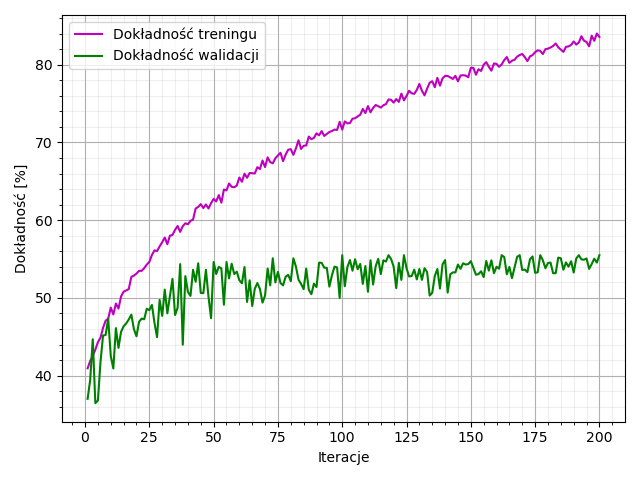
\includegraphics[width=0.7\textwidth]{wykres5.png}
    \label{pic:5.5}
\end{figure}

Tabela \ref{tab:5.10} przestawia szczegółowe wyniki osiągnięte przez tą sieć na konkretnych podzbiorach walidacyjnego zbioru danych. Tabela \ref{tab:5.11} przedstawia z kolei te same dane wyrażone w wartościach mówiących, jaki procent danych z danego podzbioru został rozpoznany jako wskazana wartość. Dla przykładu, emocje pozytywne zostały rozpoznane na 11.9\% zdjęć przedstawiających emocje negatywne. Wartości pokazują, że sieć w przypadku każdej emocji zawsze miała największe szanse na wskazanie właśnie tej właściwej. Model wykazał się szczególną dokładnością podczas analizy zdjęć negatywnych- w 68.2\% przypadkach analizy takich zdjęć uzyskano poprawny wynik. W tym miejscu warto przypomnieć, że model wytrenowany przez \cite{GAD}, który osiągał najlepszą średnią wydajność dla wszystkich emocji, osiągnął tylko 31.03\% podczas analizy emocji negatywnych, czyli aż o 37.16 p.p. mniej. Ta emocja była najczęściej udzielaną odpowiedzią w przypadku analizowanego testu- ogólnie padła w 39.4\% przypadków. Była też drugą najczęściej udzielaną odpowiedzią dla podzbiorów zdjęć pozytywnych i neutralnych, odpowiednio 25.4\% i 31.4\%. Model najsłabiej poradził sobie z rozpoznawaniem emocji neutralnych- rozpoznał je poprawnie tylko w 42.8\% przypadków analizy zdjęć przedstawiających te emocje. Może to mieć też związek z tym, że była to najrzadziej udzielana odpowiedź- zostało udzielona tylko w 26.4\% przypadków. Najczęściej popełnianym błędem pod względem ilościowym było rozpoznawanie zdjęcia pozytywnego jako negatywnego, taka błędna odpowiedź padła 444 razy, a więc w 25.4\% przypadków analizy zdjęć pozytywnych. Z kolei najczęściej popełnianym błędem w stosunku do wielkości analizowanego podzbioru, było rozpoznawania negatywnej emocji w trakcie analizy podzbioru zdjęć neutralnych- tak było w 31.3\% przypadków dla analizy tego podzbioru, a więc ogólnie 430 razy. 

\begin{table}[H]
  \centering
  \caption{Liczba rozpoznanych emocji dla konkretnych podzbiorów zdjęć.}
    \begin{tabular}{ |cc|ccc|c| }
    \hline
    \multicolumn{2}{|c|}{\multirow{2}{*}{Liczba zdjęć: 4346}} & \multicolumn{3}{c|}{Przewidywania} & \multirow{2}{*}{Suma} \\
    && Pozytywne & Neutralne & \multicolumn{1}{c|}{Negatywne} & \\
    \hline
    \multirow{3}{*}{Rzeczywiste} & Pozytywne & \textbf{986} & 317 & 444 & 1747 \\
    & Neutralne & 353 & \textbf{585} & 430 & 1368 \\
    & Negatywne & 147 & 244 & \textbf{840} & 1231 \\
    \hline
    \multicolumn{2}{|c|}{Suma} & 1486 & 1146 & 1714 & \textbf{2411} \\
    \hline
    \end{tabular}
  \label{tab:5.10}
\end{table}

\begin{table}[H]
  \centering
  \caption{Procentowy stosunek rozpoznanych emocji dla konkretnych podzbiorów danych.}
    \begin{tabular}{ |cc|ccc|c| }
    \hline
    && \multicolumn{3}{c|}{Przewidywania} & \multirow{2}{*}{Suma} \\
    && Pozytywne & Neutralne & \multicolumn{1}{c|}{Negatywne} & \\
    \hline
    \multirow{3}{*}{Rzeczywiste} & Pozytywne & \textbf{56.4\%} & 18.1\% & 25.4\% & 40.2\% \\
    & Neutralne & 25.8\% & \textbf{42.8\%} & 31.4\% & 31.5\% \\
    & Negatywne & 11.9\% & 19.8\% & \textbf{68.2\%} & 28.3\% \\
    \hline
    \multicolumn{2}{|c|}{Suma} & 34.2\% & 26.4\% & 39.4\% & \textbf{55.5\%}\\
    \hline
    \end{tabular}
  \label{tab:5.11}
\end{table}


\section{Rozszerzenie uprzednio trenowanej sieci neuronowej}
Jako ostatnie przetestowane zostanie podejście wykorzystujące transfer learning, tj. oparte na użyciu modelu wytrenowanego wcześniej na bardziej ogólnym zbiorze danych zawierającym większą liczbę klas.

Framework Keras zawiera wbudowanych kilkanaście takich modeli. Wszystkie są dostępne w pakiecie $keras.applications$. Na początku wyselekcjonowane zostaną te, które cechują się największą dokładnością w problemach zbliżonych do rozpatrywanego w tej pracy. Każdy z nich został wytrenowany wcześniej na zbiorze ImageNet \cite{ImageNet}. ImageNet to baza zdjęć zawierająca ponad 14 milionów obrazów podzielonych na tysiące klas. Z tego powodu sieci na niej trenowane cechują się dobrymi, tj. bardzo ogólnymi przestrzennymi hierarchiami cech. Do testów wytypowano 10 modeli, były to: MobileNetV2, MobileNet, NASNetMobile, VGG16, Xception, InceptionV3, ResNet50, ResNet50V2, ResNet101V2 i InceptionResNetV2.

W pierwszym teście od każdego z nich został odpięty gęsto połączony klasyfikator, a podpięty został nowy, wykorzystujący metaparametry, które najlepiej sprawdziły się w poprzednich testach. Nowy klasyfikator składał się z trzech warstw: warstwy porzucenia ze współczynnikiem równym 0.5, warstwy gęstej o 256 neuronach z funkcją aktywacji ReLU oraz warstwy gęstej o 3 neuronach, z funkcją aktywacji softmax. W procesie preprocessingu danych wszystkie zdjęcia, zarówno ze zbioru treningowego, jak i walidacyjnego, zostały skompresowane do takich samych rozmiarów, mianowicie do 150x150 pikseli. Jako funkcja straty została wykorzystana kategorialna entropia krzyżowa. Dla każdej sieci zostały przeprowadzone dwa testy, każdy z nich z wykorzystaniem innego optymalizatora. Do pierwszego testu wybrano RMSProp z learning rate równym $2\cdot10^{-5}$. W drugim teście wykorzystano optymalizator Adam z learning rate wynoszącym $2\cdot10^{-4}$.

Wyniki modeli osiągnięte na walidacyjnym zbiorze danych po przeprowadzeniu 12 cykli trenowania zostały przedstawione w tabeli \ref{tab:5.12}.

\begin{table}[H]
  \centering
  \caption{Wyniki osiągnięte przez modele wykorzystujące transfer learning}
    \begin{tabular}{ |c|c|c| }
    \hline
    Sieć & RMSProp($2\cdot10^{-5}$) & Adam($2\cdot10^{-4}$) \\
    \hline
    MobileNetV2 & \textbf{53.6\%} & \textbf{54.8\%} \\ 
    MobileNet & \textbf{52.8\%} & \textbf{53.5\%} \\ 
    NASNetMobile & 41.9\% & 42.4\% \\
    VGG16 & \textbf{56.1\%} & 43.0\% \\
    Xception & 44.3\% & \textbf{55.1\%} \\ 
    InceptionV3 & 42.4\% & 46.3\% \\
    ResNet50 & \textbf{61.1\%} & \textbf{52.4\%} \\ 
    ResNet50V2 & 40.1\% & 46.9\% \\
    ResNet101V2 & 43.9\% & 43.6\% \\ 
    InceptionResNetV2 &  41.2\% & 43.9\% \\
    \hline
    \end{tabular}
  \label{tab:5.12}
\end{table}

Do dalszych testów zostały wybrane tylko te pary modeli i optymalizatorów, których wyniki przekroczyły 50\% (zaznaczone pogrubioną czcionką). Szczególną uwagę należy zwrócić na model ResNet50, który osiągnął bardzo dobre wyniki, szczególnie przy użyciu optymalizatora RMSprop. 61.1\% to wynik mniejszy tylko o 6.5 p.p. od najlepszego wyniku osiągniętego na tej bazie danych i jednocześnie lepszy od wszystkich wyników uzyskanych w poprzednich testach, ale należy pamiętać, że ResNet50 w tym przypadku miał tylko 12 epok trenowania do dyspozycji. Sieci MobileNet i MobileNetV2 poradziły sobie zadowalająco dobrze, by warto było je dopuścić do kolejnych testów. Sieć VGG16 osiągnęła wynik nawet lepszy od nich, ale tylko przy użyciu optymalizatora RMSprop, dlatego tylko on został wykorzystany w następnych testach. Z kolei sieć Xception osiągnęła lepszy wynik z wykorzystaniem optymalizatora Adam. Można też zauważyć, że optymalizator Adam okazał się lepszy w siedmiu na dziesięć przypadków.

W kolejnym podejściu zmodyfikowano architekturę gęsto połączonego klasyfikatora. Środkowa gęsta wartwa została czterokrotnie rozszerzona, do 1024 neuronów. Zmodyfikowany został też optymalizator. Learning rate dla optymalizatora RMSProp zostało ustawiony na $2\cdot10^{-4}$, natomiast w przypadku Adam- $2\cdot10^{-3}$. Tym razem zwiększono liczbę cykli trenowania. Dokładności osiągnięte na walidacyjnym zbiorze danych po 35 iteracjach zostały przedstawione w tabeli \ref{tab:5.13}.

\begin{table}[H]
  \centering
  \caption{Wyniki osiągnięte przez najlepsze modele wykorzystujące transfer learning.}
    \begin{tabular}{ |c|c|c| }
    \hline
    Sieć & RMSProp($2\cdot10^{-4}$) & Adam($2\cdot10^{-3}$) \\
    \hline
    MobileNetV2 & 59.7\% & 58.5\% \\ 
    MobileNet & 56.7\% & 56.5\% \\ 
    VGG16 & \textbf{62.3\%} & N/A \\
    Xception & N/A & 58.5\% \\ 
    ResNet50 & \textbf{62.5\%} & 59.4\% \\ 
    \hline
    \end{tabular}
  \label{tab:5.13}
\end{table}

Tabela \ref{tab:5.13} jasno wskazuje, że sieci VGG16 i ResNet50 z optymalizatorem RMSProp osiągnęły wyniki wyraźnie lepsze od pozostałych par modeli i optymalizatorów. Jednocześnie wskazane sieci osiągały maksimum swojej wydajności w okolicach 7. epoki trenowania. Na wykresie \ref{pic:5.6} przedstawiono przykład dla modelu VGG16 wykorzystującego RMSProp z learning rate wynoszącym $2\cdot10^{-4}$. Tak szybkie osiąganie maksimum wydajności jasno wskazuje na brak potrzeby zwiększania liczby epok trenowania, a zamiast tego sugeruje konieczność skupienia się na poszukiwaniu lepszej konfiguracji gęsto zakończonego optymalizatora.

\begin{figure}[H]
    \caption{Historia dokładności w trakcie 35 iteracji uczenia dla modelu VGG16 i optymalizatora RMSProp}
    \centering
    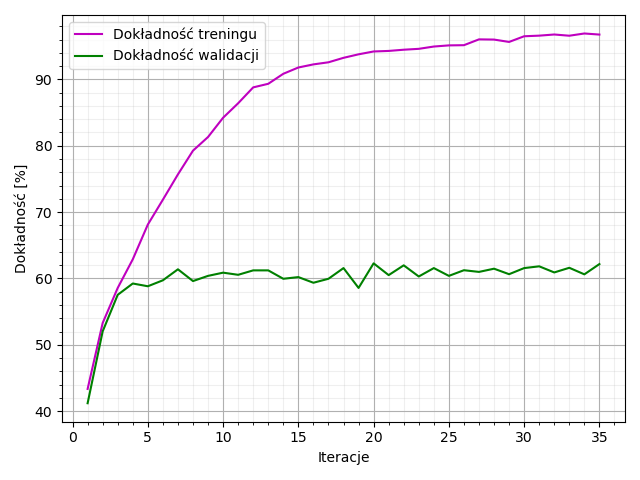
\includegraphics[width=0.7\textwidth]{wykres6.png}
    \label{pic:5.6}
\end{figure}

Kolejne testy skupiały się na różnych próbach modyfikacji gęsto połączonych klasyfikatorów modeli VGG16 i ResNet50. Punktem wyjścia był klasyfikator użyty w ostatnim teście, za pomocą którego uzyskano najlepsze wydajności (z optymalizatorem RMSProp i learning rate równym $2\cdot10^{-4}$). Pogrubioną czcionką zaznaczono sytuacje, w których udało się poprawić wyniki. Każdy test został przeprowadzany na 40 epokach treningu, a ich wyniki zamieszczono w tabeli \ref{tab:5.14}.

\begin{table}[H]
  \centering
  \caption{Wyniki osiągnięte poprzez różne wybrane modyfikacja modelu z optymalizatorem RMSProp.}
    \begin{tabular}{ |c|c|c| }
    \hline
    Modyfikacja & VGG16 & ResNet50 \\
    \hline
    Funkcja aktywacji tanh & 49.9\% & 41.3\% \\ 
    Jedna wartwa 2048 neuronów & 61.2\% & 61.3\% \\ 
    Dwie wartwy po 1024 neuronów & \textbf{62.6\%} & \textbf{62.8\%} \\ 
    Dwie wartwy po 512 neuronów & \textbf{63\%} & \textbf{63.6\%} \\
    Learning rate- $2\cdot10^{-3}$ & 52.1\% & 54.9\% \\
    Learning rate- $2\cdot10^{-5}$ & \textbf{62.7\%} & 62.2\% \\
    \hline
    \end{tabular}
  \label{tab:5.14}
\end{table}

Najlepszy wynik osiągnął model ResNet50 dla dwóch warstw złożonych z 512 neuronów, zdecydowanie przekraczając 63\%. Ogólne wyniki wskazują na to, że dodanie kolejnej wartwy gęsto połączonego klasyfikatora może pozytywnie wpłynąć na wydajność modelu, szczególnie, jeśli nowo dodana warstwa nie jest zbyt szeroka. Ponadto, dla modelu VGG16 zauważono wzrost wydajności w przypadku zastosowania optymalizatora o niższym learning rate, choć liczba iteracji potrzebnych do osiągnięcia takich wyników wynosi wtedy około 2-3 razy więcej, niż dla pozostałych rozpatrywanych przypadków.

Z tego powodu, w kolejnym teście użyto modelu VGG16 zakończonego gęsto połączonym klasyfikatorem o dwóch warstwach po 512 neuronów, z optymalizatorem RMSProp o learning rate wynoszącym $2\cdot10^{-5}$. Model osiągnął wydajność na poziomie \textbf{63.4\%}, a historię jego trenowania przedstawiono na wykresie \ref{pic:5.7}. Wynika z niego, że 40 iteracji nie było potrzebnych, ponieważ model osiągnął pełną wydajność już w połowie treningu. Sieć ResNet50 z poprzedniego testu wykorzystująca taki sam klasyfikator, ale z learning rate wynoszącym $2\cdot10^{-4}$, uzyskała wynik lepszy o 0.2 p.p., jednakże, składa się ona aż z 50 013 699 możliwych do trenowania parametrów. Dla porównania, model VGG16 jest zbudowany tylko z 19 173 699 parametrów. Ponadto, ResNet50 to sieć na tyle duża, że do przeprowadzania pojedynczej sekwencji obliczeń, nawet dla bardzo małego wsadu danych, potrzebna jest pamięć większa niż ta, jaką jest w stanie zapewnić karta graficzna Nvidia GeForce MX150. Z tego powodu obliczenia musiały być wykonywane na CPU, co w połączeniu z dużą większą liczbą parametrów koniecznych do wytrenowania sprawiło, że trening dla modelu ResNet50 zajmował około 35-40 razy więcej czasu, niż w przypadku VGG16.

\begin{figure}[H]
    \caption{Historia dokładności w trakcie 40 iteracji uczenia dla modelu VGG16 zakończonego dwiema warstwami gęstymi.}
    \centering
    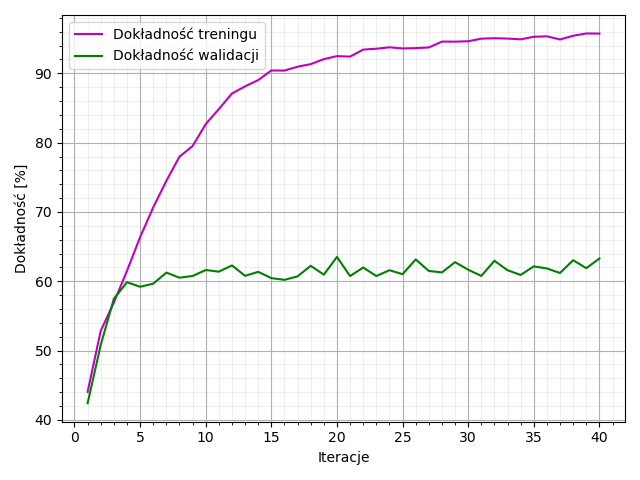
\includegraphics[width=0.7\textwidth]{wykres7.png}
    \label{pic:5.7}
\end{figure}

Niewielki rozmiar sieci VGG16 niesie ze sobą jeszcze jedną zaletę. Cały model oparty na tej bazie konwolucyjnej, wraz z wytrenowanym gęstym klasyfikatorem, po zapisaniu na dysku waży 73.1 MB. W przypadku modelu ResNet50 jest to około 2.6 razy więcej- 191 MB. Wykorzystanie mniejszego modelu skraca czas jego ładowania z dysku oraz pozwala na szybszą klasyfikację- obie te zalety mają bardzo duże znaczenie dla użytkownika końcowego. Niewielka waga modelu potencjalnie pozwala na wykorzystanie go na więcej sposobów. Dla przykładu, model o takim rozmiarze może być bez większych problemów zainstalowany na urządzeniu mobilnym- czyli sprzęcie, na którym możliwość rozpoznawania emocji na zdjęciach jest wyjątkowo pożądana z perspektywy użytkownika. %jl komercyjnego.

Podsumowując, ze wszystkich przedstawionych podejść do rozwiązania problemu, najskuteczniejszym i zapewniającym największą dokładność okazało się wykorzystanie transfer learningu. Mimo tego, że uzyskane sieci zajmują więcej miejsca na dysku, to oba te wyniki, zarówno \textbf{63.4\%} dla VGG16, jak i \textbf{63.6\%} dla ResNet50 można uznać za bardzo dobre, biorąc pod uwagę fakt, że większe, bardziej skomplikowane modele trenowane przez \cite{GAD} osiągały niewiele wyższą wydajność na zbiorze walidacyjnym. 
